\documentclass[12pt,letterpaper,addpoints,answers]{exam}
\usepackage[utf8]{inputenc}
\usepackage{amsmath}
\usepackage{amsfonts}
\usepackage{amssymb}
\usepackage{amsthm}
\usepackage{graphicx}
\usepackage{tabularx}
\usepackage[left=2cm,right=2cm,top=2cm,bottom=2cm]{geometry}
\usepackage{multicol}
\usepackage{multirow,array}
\usepackage{newtxtext,newtxmath}
\usepackage{lastpage}
\usepackage{enumitem}
\newcolumntype{Y}{>{\centering\arraybackslash}X}
\firstpageheader{}{}{
\includegraphics[scale=0.5]{BHCClogoBW.jpg}\hspace{-40pt}\vspace{-50pt}}
\firstpagefooter{}{}{Page \thepage ~of \pageref{LastPage}}
\runningheader{ \textsc{Math 181 First Exam}}{}{ \textsc{Fall 2018}}%{
\includegraphics[scale=.5]{BHCClogoBW.jpg}\vspace{-10pt}}%\hspace{-60pt}\vspace{-10pt}}
\runningheadrule
\runningfooter{}{}{Page \thepage ~of \pageref{LastPage}}
\renewcommand{\thequestion}{{\bf \arabic{question}}}
%\renewcommand{\questionlabel}{{\thequestion .}}
%\pointformat{\fbox{\themarginpoints \,pt}}
%\pointsinrightmargin
%\setlength{\rightpointsmargin}{1.5cm}
%\pointsinmargin
%\setlength{\marginpointssep}{10pt}


\begin{document}

\newcommand{\AND}{~\textsc{and}~}
\newcommand{\OR}{~\textsc{or}~}

\begin{center}
\text{ }\\
\vspace{40pt}
\textsc{{\Huge Math 181 First Exam}}\\\vspace{5pt}
\textsc{{\large Spring 2019}}\\
\vspace{60pt}
\makebox[\textwidth]{\large Name: \hrulefill{\LARGE ANSWER KEY}\hrulefill}\\
\vspace{40pt}
\fbox{\fbox{\begin{minipage}{6in}
\vspace{0.2in}
\begin{itemize}
\item Write your {\bf full name} on the line above.
\item Show your work. Incorrect answers with work can receive partial credit.
\item Attempt every question; showing you understand the question earns some credit.
\item If you run out of room for an answer, continue on the back of the page. Before doing so, write ``see back'' with a circle around it.
\item You can use 1 page (front and back) of notes.
\item You can use (and probably need) a calculator.
\item You can use the Geogebra Scientific Calculator instead of a calculator. You need to put your phone on {\bf airplane mode} and then within the application, start {\bf exam mode}; you should see a green bar with a timer counting up.
\item If a question is confusing or ambiguous, please ask for clarification; however, you will not be told how to  answer the question.
\item {\bf Box your final answer}.
\item A formula sheet is attached to this test.
\vspace{0.2in}
\end{itemize}
\end{minipage}
\begin{minipage}{0.2in}\text{ }\end{minipage}}}
\vfill
Do not write in this grade table.\\
\gradetable[h][questions]\\
\vfill
\end{center}

%%%%%%%%%%%%%%%%%%%%%%%%%%%%%%%%%%%%%%%%%%%%%%%%%%%%%%%%%%%%%%%%%%%%%%%%%%%%%%%

\newpage

\rhead{\textsc{Definitions and Formulas}}
{\bf Sample statistics:}\vspace{-10pt}
\begin{multicols}{2}\noindent
$n=\text{sample size} $\\
$x_i=\text{the $i$th value in a sample} $\\
$\bar x = \text{sample mean}$\\
$s = \text{sample standard deviation}$\\\\
$\bar x = \cfrac{\sum\limits_{i=1}^n x_i}{n}$

\columnbreak \noindent
$Q_1$ = first quartile\\
$m$ = median\\
$Q_3$ = third quartile\\
IQR = inter-quartile range = $Q3-Q1$\\\\
$s = \sqrt{\cfrac{\sum\limits_{i=1}^n (x_i-\bar x)^2}{n-1}}$ 
\end{multicols}

{\bf Population parameters:}\\
$\mu = \text{population mean}$\\
$\sigma = \text{population standard deviation}$\\

{\bf Probability:}
\begin{multicols}{2} \noindent
$\Omega = \text{set of all possible equally likely outcomes}$\\
$A = \text{event A, a set of outcomes}$\\
$A^c = \text{The complement of }A$\\
$B = \text{event B, another set of outcomes}$\\
$\#(A) = \text{size of set, number of outcomes in } A$\\
$P(A) = \text{probability of }A$\\
$P(A \AND B) = \text{probability of both $A$ and $B$}$\\
$P(A \OR B) = \text{probability of either $A$ or $B$ (or both)}$\\
$P(A | B) = \text{probability of $A$ given $B$}$\\
$\iff = \text{``if and only if''}$
\columnbreak

$$P(A) = \cfrac{\#(A)}{\#(\Omega)}$$
$$0 \le P(A) \le 1$$
\begin{align*}
P(A \AND B) &= P(A) \cdot P(B|A) \\
P(A \OR B) &= P(A) + P(B) - P(A\AND B)\\
P(A|B) &= \frac{P(A \AND B)}{P(B)} \\
P(A^c) &= 1 - P(A)
\end{align*}
\end{multicols}

\noindent
$A$, $B$ are disjoint (mutually exclusive) ~~$\iff~~P(A\AND B) = 0$\\
$A$, $B$ are non-disjoint ~~$\iff~~P(A\AND B) > 0$\\
$A$, $B$ are exhaustive ~~$\iff~~P(A\OR B) = 1$\\
$A$, $B$ are complements ~~$\iff$~~ $A$, $B$ are disjoint and exhaustive ~~$\iff$~~ $B=A^c$\\
$A$, $B$ are independent ~~$\iff~~P(A\AND B) = P(A)\times P(B) ~~\iff~~ P(A|B)=P(A)$\\

{\bf Random variables and distributions:}\\
$X=$ random variable \\
$x_i=$ the $i$th possible value of $X$. (Notice different meaning here {vs.} sample statistics.)\\
$k=$ number of possible values of $X$.\\
$E(X)=\mu=$ expected value of $X$\\
$\sigma=$ standard deviation of $X$
$$\mu = \sum\limits_{i=1}^k  x_i \cdot P(X=x_i) $$\\
$$\sigma = \sqrt{\sum\limits_{i=1}^k (x_i-\mu)^2 \cdot P(X=x_i)}$$


\newpage
\lhead{\textsc{Math 181}}
\rhead{\textsc{First Exam}}
\begin{questions}
\question[10] Samuel suspects that coffee impairs short-term memory. Samuel runs a study by asking random BHCC students to participate in a memory challenge: repeating back 7 random digits. Samuel marks whether the participant successfully repeated the digits. Then, Samuel asks the participant whether they had coffee in the last 3 hours. The results are summarized below.

\begin{center}
\begin{tabular}{c|c c|c}
          & success & fail & total \\ \hline
coffee    &  16   & 7      & 23   \\
no coffee &  11   & 4      & 15   \\ \hline
total     &  27   & 11     & 38
\end{tabular}
\end{center}

\begin{parts}
\part What kind of study was this?
\begin{checkboxes}
\choice experimental
\CorrectChoice observational
\end{checkboxes}
\begin{solution}
There was no assignment to groups.
\end{solution}

\part Which group performed better (had a higher proportion of success)?
\begin{checkboxes}
\choice coffee
\CorrectChoice no coffee
\end{checkboxes}
\begin{solution} You need to find the proportion of each group.
$$\frac{16}{23} = 0.696$$
$$\frac{11}{15} = 0.733$$
\end{solution}

\part Which hypothesis is the null hypothesis?
\begin{checkboxes}
\CorrectChoice The difference in proportions is due to chance.
\choice The difference in proportions is due to an association between coffee and memory.
\end{checkboxes}
\vfill
\part Which hypothesis is the alternative hypothesis?
\begin{checkboxes}
\choice The difference in proportions is due to chance.
\CorrectChoice The difference in proportions is due to an association between coffee and memory.
\end{checkboxes}
\vfill
\part Would you reject the null hypothesis? Why?
\begin{checkboxes}
\choice Yes. The difference seems too large for chance.
\CorrectChoice No. The difference seems small enough to be just from chance.
\end{checkboxes}
\vfill
\end{parts}

\begin{solution} With enough thought, these choices should give you the answers to the previous two questions...
\end{solution}

\newpage

\question[8] When ``acoustic guitar'' was searched on craigslist, there were 144 local postings that included a price.  These prices are displayed as a histogram.
\vspace{-0.3in}
\begin{center}
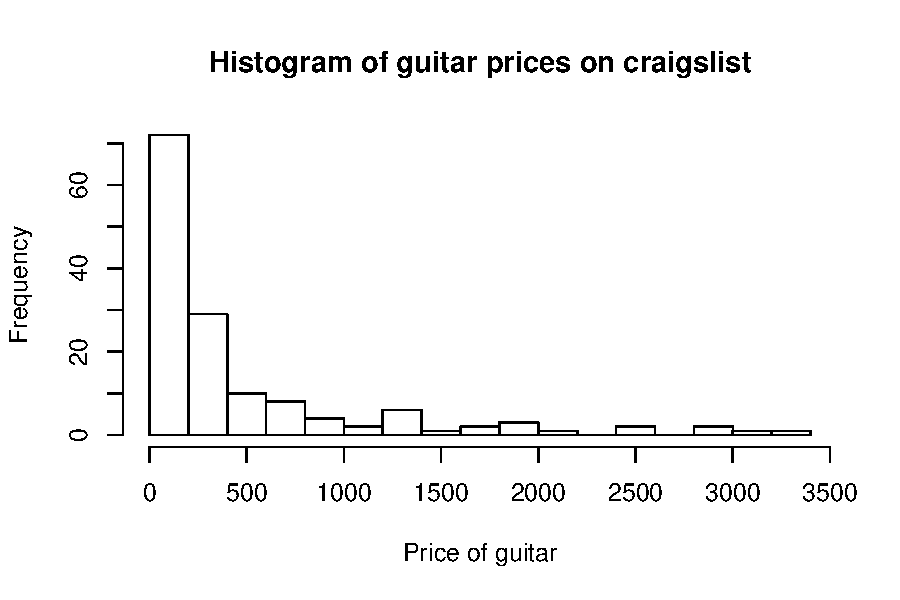
\includegraphics[scale=0.9]{figures/guitars.pdf}
\end{center}
\begin{parts}

\part Which of the following would be an appropriate estimate of the median?
\\\begin{oneparcheckboxes}
\choice \$1
\CorrectChoice \$200
\choice \$500
\choice \$3500
\end{oneparcheckboxes}
\begin{solution}
The class 0-200 has almost exactly 72 prices, which is half of the 144 prices. You could have also seen the 15-price sample has a similar median.
\end{solution}

\part Which of the following would be an appropriate estimate of the mean?
\\\begin{oneparcheckboxes}
\choice \$1
\choice \$200
\CorrectChoice \$500
\choice \$3500
\end{oneparcheckboxes}
\begin{solution}
We know the mean should be higher than the median because of the right skew. Also, you could have used the 15-price sample to inform this. 
\end{solution}

\part Which of the following would be an appropriate estimate of the standard deviation?
\\\begin{oneparcheckboxes}
\choice \$1
\choice \$20
\CorrectChoice \$700
\choice \$3500
\end{oneparcheckboxes}
\begin{solution}
Standard deviation is approximately the average deviation from the mean. It can also be thought of as a typical amount of spread. The standard deviation is often about 1/6 of the range. You could have also calculated the standard deviation of the 15-price sample. 
\end{solution}

\part Which option best describes this histogram?
\begin{checkboxes}
\choice Skew-left
\CorrectChoice Skew-right
\choice Superstitious
\choice Symmetric
\end{checkboxes}
\end{parts}


\newpage

\question[8] From the guitar prices, a random sample of size 15 was taken. Those 15 prices are listed below.

\begin{center}
\begin{tabular}{c c c c c c c c c c c c c c c}
10&20&60&60&75&85&125&150&220&250&275&700&1395&1800&2000
\end{tabular}
\end{center}

\\
Make a boxplot summarizing these data. Be sure to indicate $Q_1$, $Q_3$, median, outliers, and ends of whiskers. The axis below is meant to help you. 

\begin{solution}
median = 150 ; Q1 = 60 ; Q3 = 700 ; IQR = 640 \\
check for outliers:
\\ 60-1.5*640 = -900
\\ 700+1.5*640 = 1660
\end{solution}
\vfill 
\\ \hfill
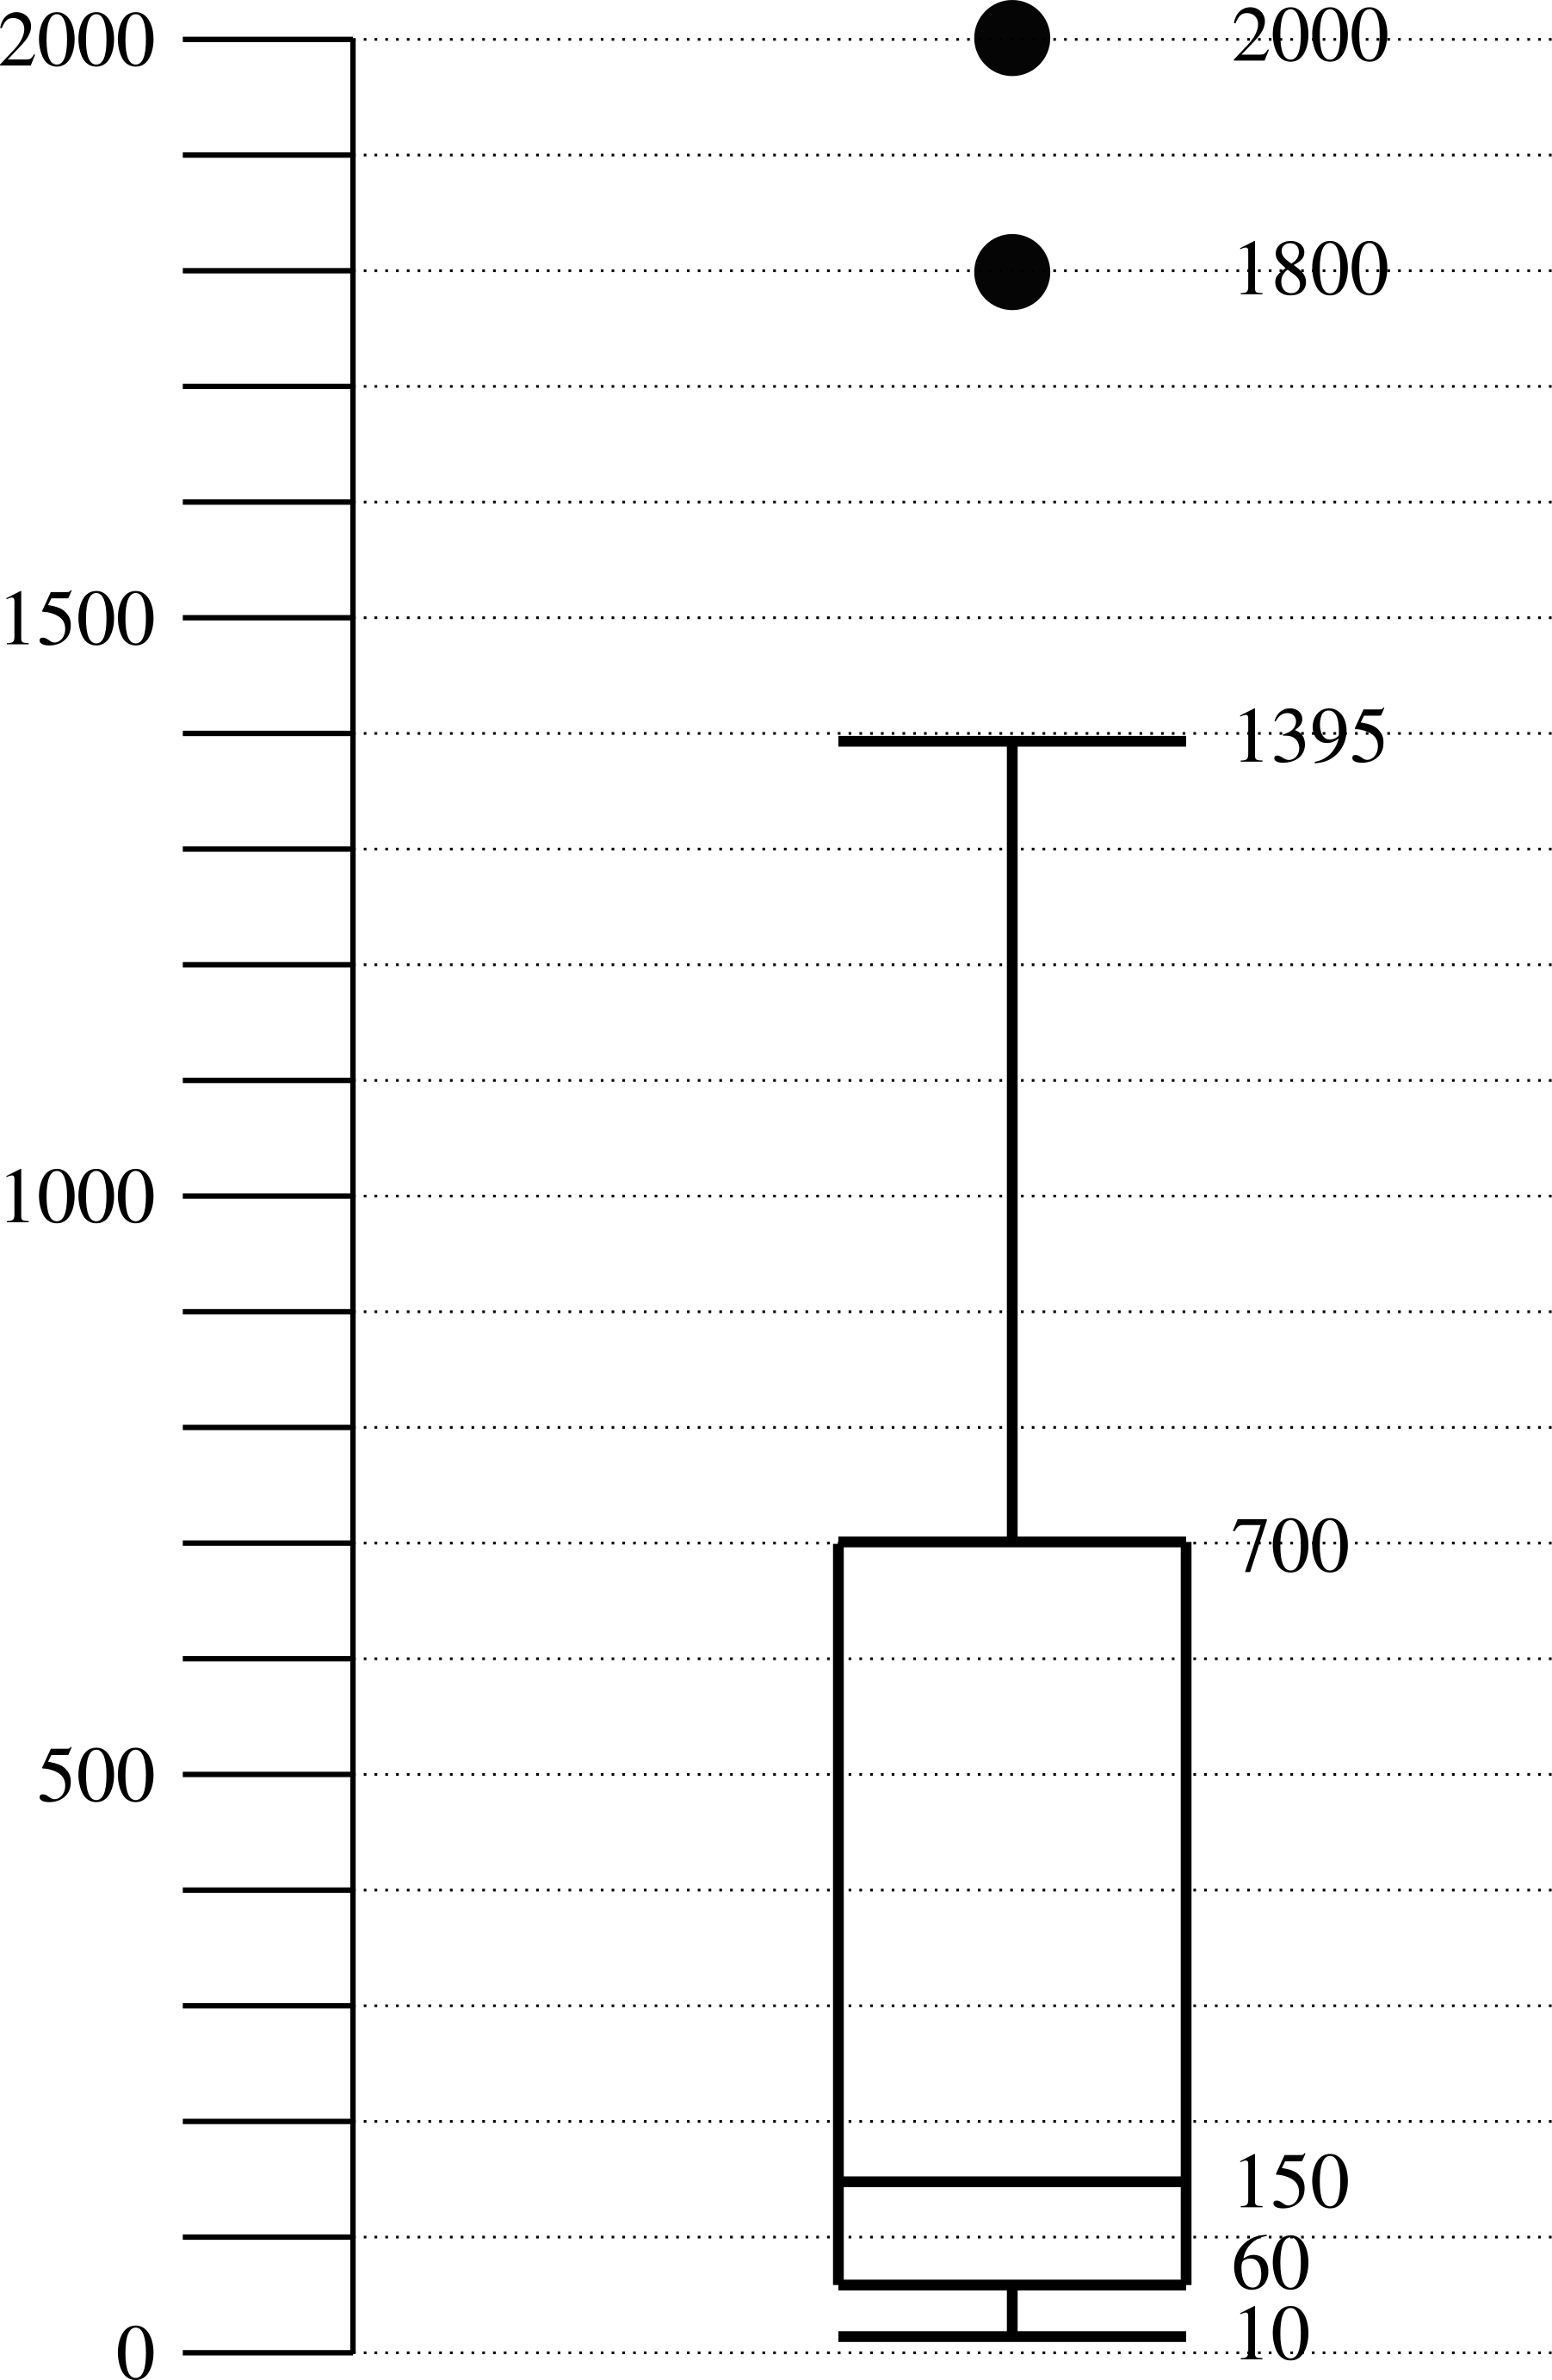
\includegraphics[scale=0.7]{figures/boxplot_axis_answer.png}


\newpage 

\question[16] A jar contains 99 marbles. Each marble has a color and a pattern. The frequencies are shown in the contingency table.
\begin{center}
\begin{tabularx}{0.6\textwidth}{|Y|Y Y Y|Y|}\hline
          & red & green & blue & total\\ \hline
dotted    & 7  & 8  & 9 & 24 \\
striped   & 10 & 11 & 12 & 33 \\
checkered & 13 & 14 & 15 & 42  \\ \hline
total     & 30 & 33 & 36 & 99 \\ \hline
\end{tabularx}
\end{center}
\begin{parts}
\part What is the probability that a random marble is green?
\begin{solution}
$\frac{33}{99} \approx 0.33 $
\end{solution}
\part What is the probability that a random marble is checkered?
\begin{solution}
$\frac{42}{99} \approx 0.42 $
\end{solution}
\part What is the probability that a random marble is either striped {\bf or} green (or both)?
\begin{solution}
$\frac{33+33-11}{99} \approx 0.56 $
\end{solution}
\part What is the probability that a random marble is both red {\bf and} dotted?
\begin{solution}
$\frac{7}{99} \approx 0.07 $
\end{solution}
\part What is the probability that a random marble is red {\bf given} it is checkered?
\begin{solution}
$\frac{13}{42} \approx 0.31 $
\end{solution}
\part What is the probability that a random marble is striped {\bf given} it is blue?
\begin{solution}
$\frac{12}{36} \approx 0.33 $
\end{solution}
\part When picking one random marble, which two events are disjoint (mutually exclusive)?
\\\begin{oneparcheckboxes}
\choice red, checkered
\choice green, striped
\CorrectChoice blue, red
\end{oneparcheckboxes}
\begin{solution}
$P(B \AND R) = 0$
\end{solution}
\part When picking one random marble, which two events are independent?
\\\begin{oneparcheckboxes}
\choice red, checkered
\CorrectChoice green, striped
\choice blue, red
\end{oneparcheckboxes}
\begin{solution}
$P(G \AND S) = P(G) \cdot P(S)$
\end{solution}
\end{parts}

\newpage

\question[9] Let random variable $X$ represent the number of tails showing when four fair coins are flipped. The probability distribution of $X$ is shown below, where $x_i$ represents the $i$th possible value of $X$.
\begin{center}
\begin{tabular}{|c|c|} \hline
$x_i$ & $P(X=x_i)$ \\ \hline
0 & 0.0625 \\
1 & 0.25 \\
2 & 0.375 \\
3 & 0.25 \\
4 & 0.0625 \\ \hline
\end{tabular}
\end{center}
\begin{parts}
\part What is the probability of 2 tails? In other words, evaluate $P(X=2)$.
\begin{solution} 
$$0.375$$
\end{solution}
\vfill
\part What is the probability of at least 2 tails? In other words, evaluate $P(X \ge 2)$.
\begin{solution} 
$$0.375 + 0.25 + 0.0625 = \fbox{0.6875}$$
\end{solution}
\vfill
\part What is the probability of more than 2 tails? In other words, evaluate $P(X > 2)$.
\begin{solution} 
$$0.25 + 0.0625 = \fbox{0.3125}$$
\end{solution}
\vfill
\bonuspart[2] Determine $x$ such that $P(X<x)=0.9375$ and $P(X > x)=0$.
\begin{solution} 
Notice that $$P(X<4) = 0.0625+0.25+0.375+0.25 = 0.9375 $$
and
$$P(X>4) = 0 $$
Thus, $$x=4$$
\end{solution}
\end{parts}

\newpage

\question[9] A machine cuts rods to 30 centimeters. However, the machine is not perfect, so the actual lengths have variability. 

Let the continuous random variable $Y$ represent the length of a rod. An engineer determines $Y$ approximately follows the distribution shown by the density function below. The entire area under the curve is 100\%, and each square is worth 1\%.

\begin{center}
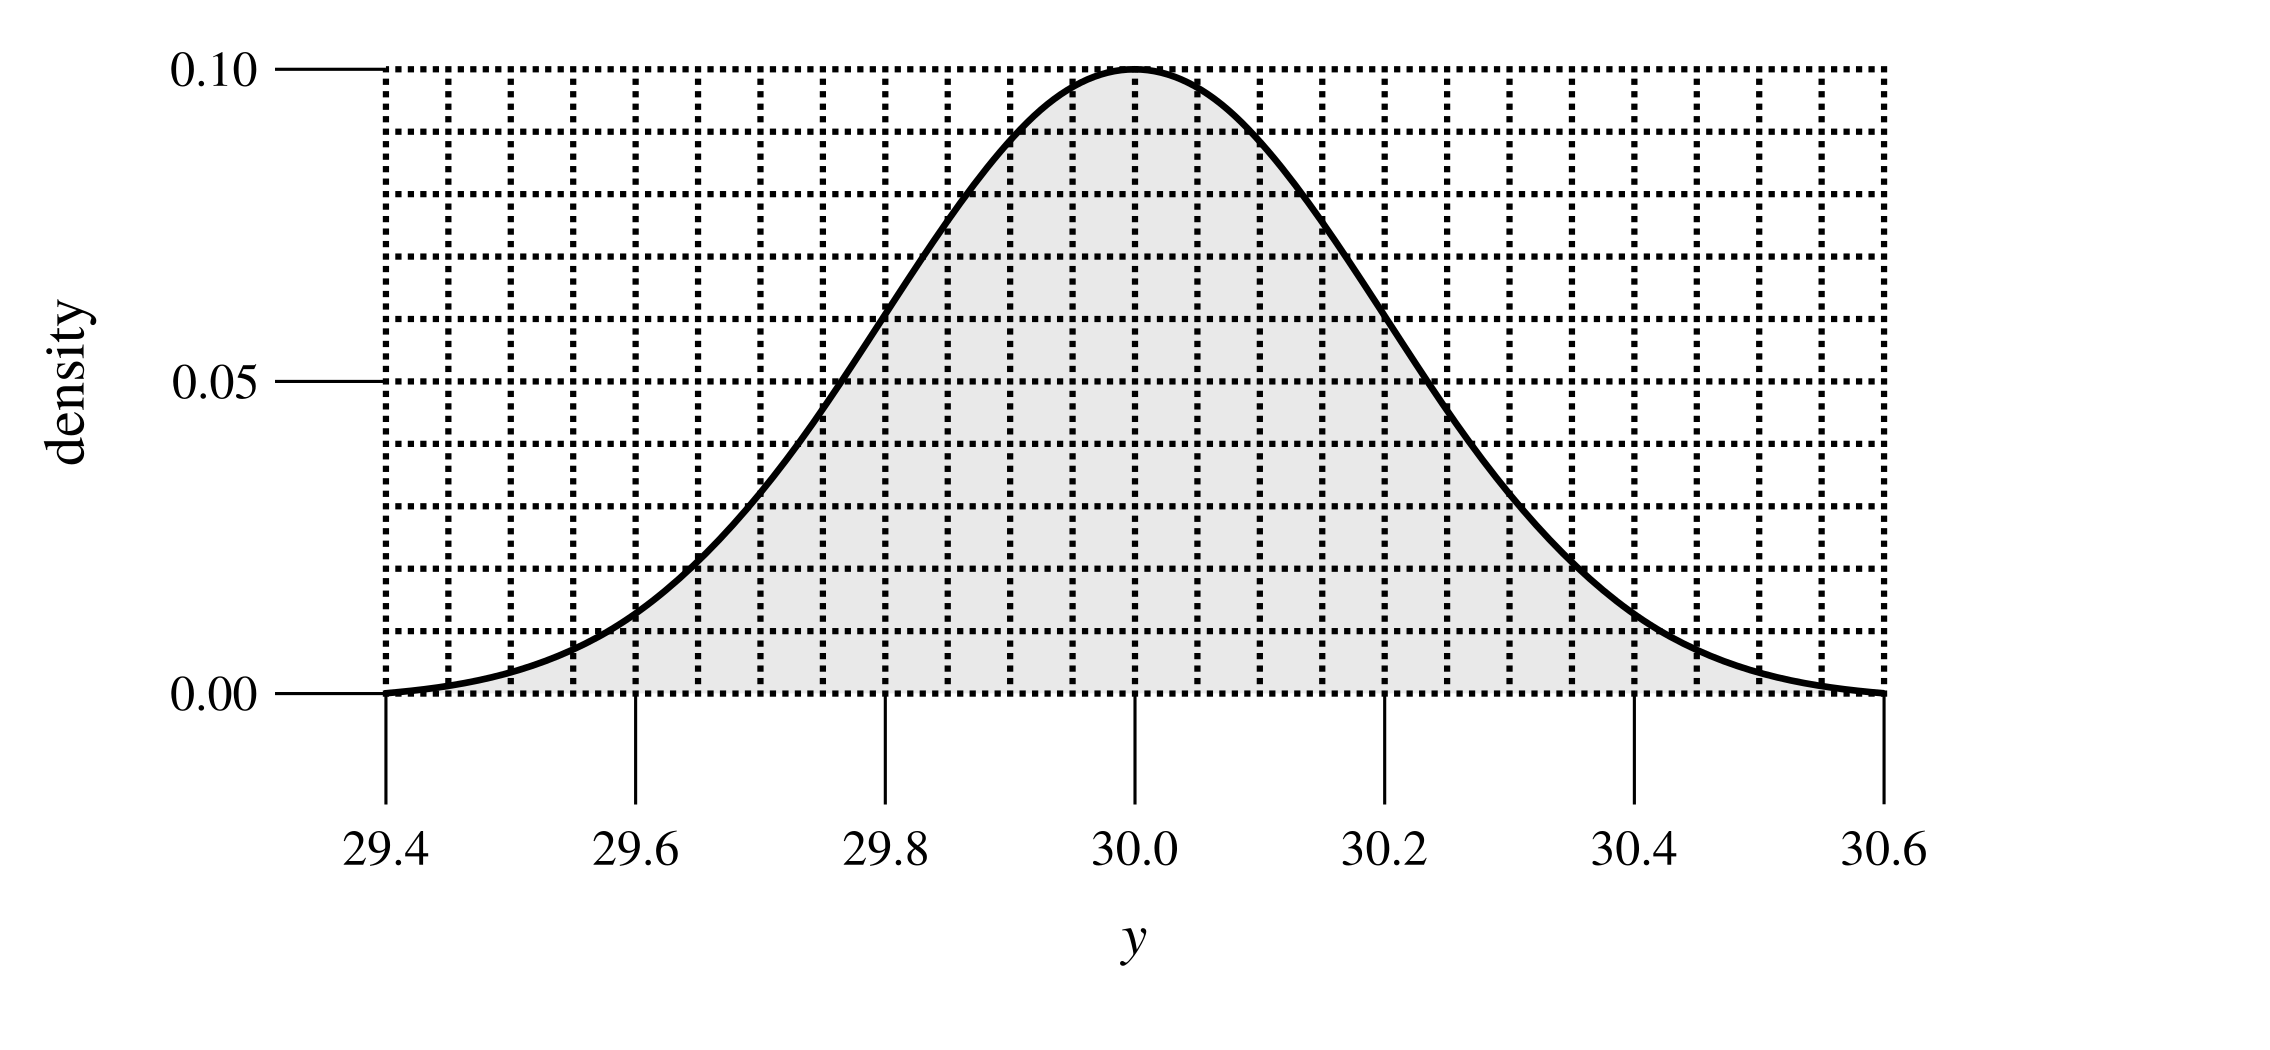
\includegraphics[scale=0.95]{figures/norm2.png}
\end{center}
\begin{parts}
\part Estimate the probability a rod is cut to exactly 30.2 centimeters.\\ In other words, estimate $P(Y=30.2)$.
\begin{solution} 
A continuous random variable will never exactly hit a specific number. Remember, we find areas to find probabilities. A rectangle with no width has no area.
$$0$$
\end{solution}
\part Estimate the probability a rod is cut to a length between 30.2 centimeters and 30.4 centimeters?
\\ In other words, evaluate $P(30.2 < Y < 30.4)$.
\begin{solution} 
If you count the squares under the curve from 30.2 until 30.4, you should count about 13 or 14 squares (I guess 12 is fine too).
$$13\% ~\text{or}~ 14\%$$
\end{solution}
\part Estimate $Q_1$, the 25th percentile. Answers within $\pm 0.02$ will count.
\\In other words, estimate $Q_1$ such that $P(Y < Q_1)=0.25$.
\begin{solution} 
Start counting from the left until you reach 25\%. Your answer should be between 29.85 and 29.90.
\end{solution}



\end{parts}
\end{questions}
\end{document}
